The conversion process used by \texfourht\ involves several tools
(see section \ref{sec:overview}, \nameref{sec:overview} for details). 


We provide a build script, called \shellcmd{make4ht}, which simplifies the 
process.


\section{\texttt{make4ht} Build System}
\label{sec:make4ht-intro}

The conversion command loads a script which takes on itself to invoke the
different steps of the process, without user intervention. The command assumes
the form:

\begin{shellcommand}
make4ht [make4ht options] filename.tex "options1" "option2" "options3" "options4"
\end{shellcommand}

The first set of options is for the tex4ht.sty and *.4ht style files, the
second set is for the tex4ht post-processor, the third for the t4ht
post-processor, and the last one is for the \LaTeX\ compiler. 

These options are optional.

The basic invokation of make4ht looks like this:

\begin{shellcommand}
make4ht filename.tex
\end{shellcommand}

This command requests a translation according to the default conditions, which are set to produce HTML 5 document.

\begin{shellcommand}
make4ht filename.tex "2,info"
\end{shellcommand}

This command specifies some options for tex4ht.sty. The "2" option requests a
break up of the output into separate web pages, in accordance to the two top
sectioning levels of the document.

The \texttt{info} option requests inclusion of documentation of basic configurations to the \texttt{filename.log} file.
You can open this file using a text editor to read this information.

Information about additional options can be found in the \namerefpage{sec:texfouhtoptions} section.



\begin{shellcommand}
make4ht -c foo.cfg filename "frames" "" "-p"
\end{shellcommand}

This command requests LaTeX to load a \nameref{sec:private-configuration}, named
foo.cfg, using the \texttt{-c} make4ht option. The \texttt{frames} option
requires placing of the content and table of contents in separate frames. In
addition, it asks the \shellcmd{t4ht} command not to produce bitmaps for pictures using the \shellcmd{-p} option.

\section{\makefourht{} Switches and Options}

\makefourht{} accepts following command line switches and options:

\begin{textsource}
-a,--loglevel (default status) Set log level.
possible values: debug, info, status, warning, error, fatal
-b,--backend (default tex4ht) Backend used for xml generation. 
possible values: tex4ht or lua4ht
-c,--config (default xhtml) Custom config file
-d,--output-dir (default nil)  Output directory
-e,--build-file (default nil)  If build file is different than `filename`.mk4
-f,--format  (default html5)  Output file format
-h,--help  Display this message
-j,--jobname (default nil)  Set the jobname
-l,--lua  Use lualatex for document compilation
-m,--mode (default default) Switch which can be used in the makefile 
-n,--no-tex4ht Disable dvi file processing with the tex4ht command
-s,--shell-escape Enables running external programs from LaTeX
-u,--utf8  [obsolete] The document is generated in UTF8 encoding by default
-v,--version  Display version number
-x,--xetex Use xelatex for document compilation
\end{textsource}

You can either use the long form \shellcmd{--mode}, or the short form \shellcmd{-m}. 
Short options can be chained:

\begin{shellcommand}
$ make4ht -lsm draft filename.tex
\end{shellcommand}

The above command is equvalent to the following that uses the long names:

\begin{shellcommand}
$ make4ht --lua --shell-escape --mode draft filename.tex
\end{shellcommand}

Some of these options are discussed in other chapters, see section \namerefpage{sec:private-configuration}
for details on configuration files requested using the \shellcmd{-c} option,
and section \namerefpage{sec:make4ht-build-files} for details on build files requested using 
the \shellcmd{-e} option.

Supported  output formats are described in the chapter \ref{sec:output-formats}. They can be requested using the \shellcmd{-f} option.
This option also supports extensions. This feature was shown in the section \namerefpage{sec:tutorial-basic-usage} of the tutorial.

\subsection{Terminal Output}

\makefourht\ hides the terminal output by default. It shows only errors and warnings.
It doesn't always show the correct error context. In such cases, try the \shellcmd{-a debug} option.
It is also recommended to use output of this option for \TeX4ht bug reports.

\begin{shellcommand}
$ make4ht -a debug -m draft buggy.tex
\end{shellcommand}


\subsection{Output Directory}

To copy generated files to a different directoy, use the \shellcmd{-d path} option. The passed path
can be absolute or relative to the current directory. It also doesn't need to exist, \makefourht{}
will create it if necessary.

\begin{shellcommand}
$ make4ht -d outdir filename.tex
\end{shellcommand}

Note that this option doesn't remove any files from the current directory. If you want to remove the temporary
files, use the \shellcmd{-m clean} option:

\begin{shellcommand}
$ make4ht -m clean filename.tex
\end{shellcommand}


\section{Overview of the Translation Process}\label{sec:overview}


The translation of a LaTeX source file into HTML involves loading of
the \texttt{tex4ht.sty} package. It watches loaded packages, and loads
corresponding configuration files, named as \texcommand{<pkgname>.4ht}. 
These configuration files patches commands provided by the packages, and
insert special hooks, which are later filled with XML code for the output format.

To ensure that all packages are processed, \texttt{tex4ht.sty} needs to be 
loaded early, ideally before \texcommand{\documentclass}.

Result of the \LaTeX{} run is a DVI file that contain document text and 
special instructions with XML code, or with requests for pictures. 
This file is then processed by the \shellcmd{tex4ht} command. It generates
the output XML or HTML files and the IDV file, which is then used for 
pictures. 

The last command is \shellcmd{t4ht}. It generates pictures and CSS file.

Basic sequence of execution of these command is following:

\begin{shellcommand}
latex      x            (or ‘tex x’) 
latex      x 
latex      x 
tex4ht     x 
t4ht       x 
\end{shellcommand}

The three compilations with La(\TeX) are needed to ensure proper links. The approach is illustrated in the picture \ref{fig:process}. 

\begin{figure}
  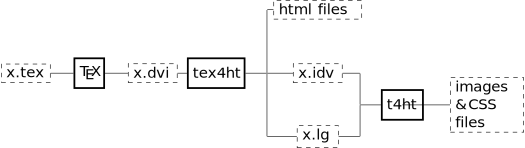
\includegraphics[width=\textwidth]{images/tex4ht_process/tex4ht_process}
  \caption{\texfourht\ process overview}
  \label{fig:process}
\end{figure}

\begin{description}
  \item[x.tex]

This is a source TeX/LaTeX/OtherTeX file that imports the style files tex4ht.sty and *.4ht. The style files define the features for the output.

\item[tex4ht]

The output of \TeX{} is a standard dvi file interleaved with special
instructions for the postprocessor \shellcmd{tex4ht} to use. The special
instructions come from implicit and explicit requests made in the source file
through commands of \texfourht.

The utility tex4ht translates the dvi code into standard text, while obeying
the requests it gets from the special instructions. The special instructions
may request the creation of files, insertion of html code, filtering of
pictures, and so forth.

In the extreme case that the source code contains no commands of \TeX4ht, it
gets the pure dvi code and it outputs (almost) plain text with no hypertext
elements in it.

The special (\texcommand{\special}) instructions seeded in the DVI code are not understood
by dvi processors other than those of \TeX4ht.

\item[x.idv]

This is a dvi file extracted from x.dvi, and it contains the pictures needed in
the html files.

\item[x.lg]

This is a log file listing the pictures of x.idv, the png files that should be
created, CSS information, and user directives introduced through the
‘\texcommand{\Needs{...}}’ command.

\item[t4ht]
This is an interpreter for executing the requests made in the x.lg script.

\end{description}

\subsection{make4ht extensions}\label{sec:make4ht-extensions}
